Here, we propose a spectroscopic method for probing the qubit transition frequency using an echo-root-Lorentzian drive pulse. Previous theoretical work showed that Lorentzian pulses exhibit power narrowing, complementary to the conventional power broadening observed for constant drives, as a consequence of their adiabatic properties~\cite{boradjiev_power_2013}. Power narrowing with powers-of-Lorentzian pulses was subsequently demonstrated experimentally on IBM Quantum, including the cutoff broadening introduced by truncating the pulse wings~\cite{mihov_defying_2024}. In this work, we extend this framework to longer pulse durations approaching the $T_1$ timescale and introduce a $\pi$-phase jump at the pulse peak. The resulting echo property effectively cancels the net pulse area while preserving the adiabatic properties of the drive. This phase inversion reverses the coherent phase accumulation at resonance, suppressing on-resonant excitation while maintaining an off-resonant spectral response across the frequency domain, and thus making resonance distinguishable.

\begin{figure*}[t]
    \centering
    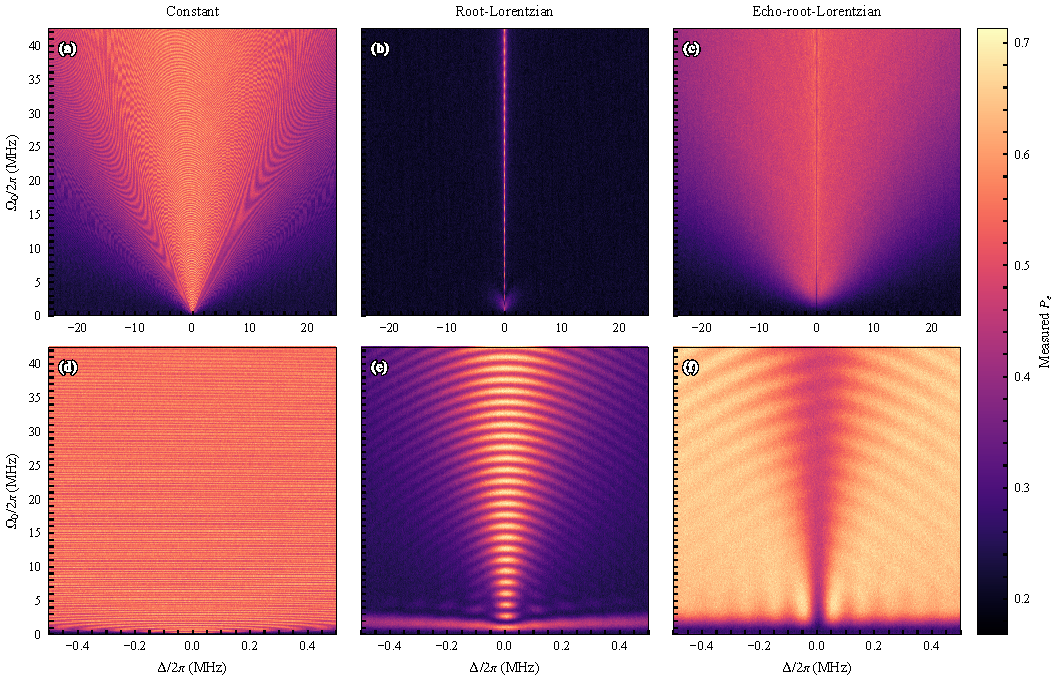
\includegraphics[width=0.92\textwidth]{../figures/paper/02_central_spectroscopy.pdf}
    \caption{
Experimental q1 spectroscopy maps for $20~\mu\mathrm{s}$ pulses.  The color
scale is the state-discriminated, measured excited-state population $P_e$.
The upper row shows the broad $100~\mathrm{MHz}$ domain ($-50$ to
$+50~\mathrm{MHz}$) with $0.5~\mathrm{MHz}$ spacing; the lower row shows the
narrow $1~\mathrm{MHz}$ domain ($-0.5$ to $+0.5~\mathrm{MHz}$) with
$5~\mathrm{kHz}$ spacing.  From left to right, the columns show a nearly
constant-envelope echo implemented as a root-Lorentzian with a
midpoint phase inversion, an ordinary root-Lorentzian with $c=0.005$, and an
echo-root-Lorentzian with $c=0.005$.  All broad maps and the narrow
constant-envelope map contain 200 shots per point.  The narrow ordinary-pulse
run contains 216 completed averages per point despite requesting 1000, while
the narrow echo-root-Lorentzian run contains all 1000.  All panels use
the same 200-point calibrated peak-Rabi grid, extending from zero to
approximately $25.1~\mathrm{MHz}$, and the same probability scale.  Active
reset and state-discriminated readout are used throughout.
The white dashed line denotes the programmed zero detuning.
    }
    \label{fig:robust-echo-spectroscopy}
\end{figure*}

\begin{figure}[t]
    \centering
    
\includegraphics[width=\columnwidth]{%
        ../figures/paper/03_lorentzian_echo_slices.pdf}
    \caption{Experimental and simulated spectra.
    (a)--(f) Final excited-state probability $P_e$ versus detuning for
    $20~\mu\mathrm{s}$ root-Lorentzian (left) and echo-root-Lorentzian (right)
    pulses with $c=0.005$.  From top to bottom,
    $\Omega_0/2\pi=3$, $20$, and $40~\mathrm{MHz}$. Continuous lines show
    three-level simulations and markers show experiment. A common global
    population offset and small gain adjustment are applied to the measured
    traces for comparison. Residual baseline mismatches remain, but the
    spectral profiles otherwise agree closely. At high drive, the echo
    response shows a line-shape discrepancy and a deeper experimental
    resonance dip, providing a stronger signal for resonance detection.
    Partial refocusing of slowly varying, non-Markovian noise by the echo
    is a possible explanation for the enhanced dip contrast relative to the
    Markovian model, consistent with noise suppression in rotary-echo
    experiments~\cite{gustavsson_rotary_echo_2012}.
    }
    \label{fig:simulation-results}
\end{figure}


We define the echo-root-Lorentzian drive from the order-$n$ generalized
Lorentzian envelope as
\begin{align}
L^{(n)}(t)
&= \frac{1}{\left[1+\left(\frac{t}{\tau}\right)^2\right]^n},
\\
L^{(1/2)}_{\mathrm{echo}}(t)
&:= L^{(1/2)}(t)\,\mathrm{sgn}(t).
\label{eq:Ln}
\end{align}
where $\tau$ sets the characteristic pulse duration and $n$ controls the
algebraic decay of the wings.

For the untruncated, plain generalized Lorentzian with $n>1/2$, the boundary of
adiabatic following provides an estimate of the characteristic spectral width.
Applying the usual adiabatic condition to this envelope gives~\cite{boradjiev_power_2013}
\begin{equation}
\Delta_b\tau
\propto
(\Omega_0 \tau)^{-\frac{1}{2n-1}},
\label{eq:lorentzian_adiabatic}
\end{equation}
where $\Delta_b$ is the angular detuning at which adiabatic following ceases
and $\Omega_0$ is the peak angular Rabi frequency.  Because the exponent is
negative, this characteristic detuning decreases as the drive strength
increases, producing power narrowing rather than conventional power broadening.
The exponent grows without bound as $n\to1/2^+$, so within its domain this
asymptotic result predicts the steepest narrowing trend at the root-Lorentzian
boundary.  At $n=1/2$, finite truncation, decoherence, and the echo phase
inversion regularize the response, and the FWHM $\Gamma_f$ used below is
therefore obtained from the complete experimental spectrum.  This
interpretation is consistent
with the power narrowing and cutoff broadening observed for powers of
Lorentzian pulses by Mihov and Vitanov~\cite{mihov_defying_2024}.  In contrast,
a square pulse exhibits conventional power broadening, with
$\Gamma_\omega\propto\Omega_0$ at large drive.  The derivation and the marginal
$n=1/2$ limit are detailed in the Supplemental Material~\cite{SupplementalMaterial}.
